\section{Résultats des métriques}
  L'intervalle entre chaque batch a été fixé à 1 seconde. Ainsi, Spark va récupérer pendant 1 seconde les tweets grâce à l'API de Twitter, effectuer les opérations de statistiques sur ces tweets et restituer l'information, dans notre cas, sous forme d'affichage à l'écran. Un diagramme de déploiement est présenté à la figure \ref{fig:digramme de déploiement}.

    \begin{figure}
        \centering
        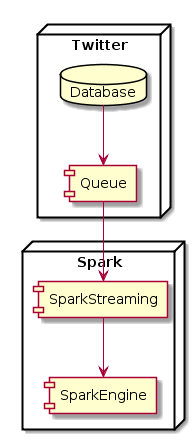
\includegraphics{images/diagramme-deploiement.png}
        \caption{Diagramme de déploiement}
        \label{fig:digramme de déploiement}
    \end{figure}

  \subsection{Time behaviour}
    Une des catégories de métriques est la notion de temps. En effet, pour l'analyse en temps réel, il est nécessaire de connaître les durées de chaque action afin de déterminer d'éventuel goulot d'étranglement. Pour notre prototype, nous avons mis en place une métrique sur la durée pour effectuer un batch complet, à savoir la récupération des tweets et le calcul de statistiques sur celui-ci. Une deuxième métrique a été mise en place dans le but de relever la durée nécessaire seulement pour réaliser les statistiques sur les tweets d'un batch. La figure~\ref{fig:resultats_stat_tweet} présente les résultats obtenus. \\

    \begin{figure}
      \centering
      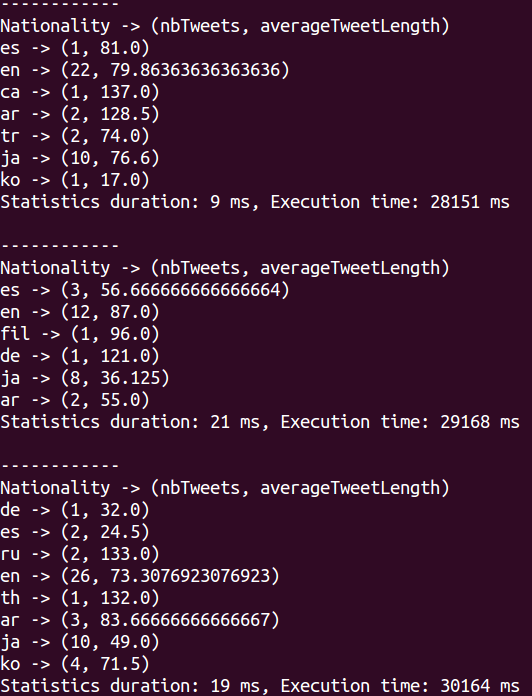
\includegraphics[width=0.6\textwidth]{images/stat_results.png}
      \caption{Résultats de l'analyse de tweet en temps réel}
      \label{fig:resultats_stat_tweet}
    \end{figure}

    Nous pouvons observer trois batch différents. Cela correspond donc à un temps d'exécution théorique de streaming de trois secondes (car nous avions spécifié un intervalle de 1 seconde comme paramètre). Cela est confirmer d'un point de vue exécution grâce à la métrique \emph{Execution time} présent sur la figure~\ref{fig:resultats_stat_tweet}. Nous pouvons remarquer que cette métrique prend respectivement les valeurs 28151, 29168 et 30164 millisecondes. Il y a donc bien 1 seconde entre chaque retour de résultats. \\

    \begin{figure}
      \centering
      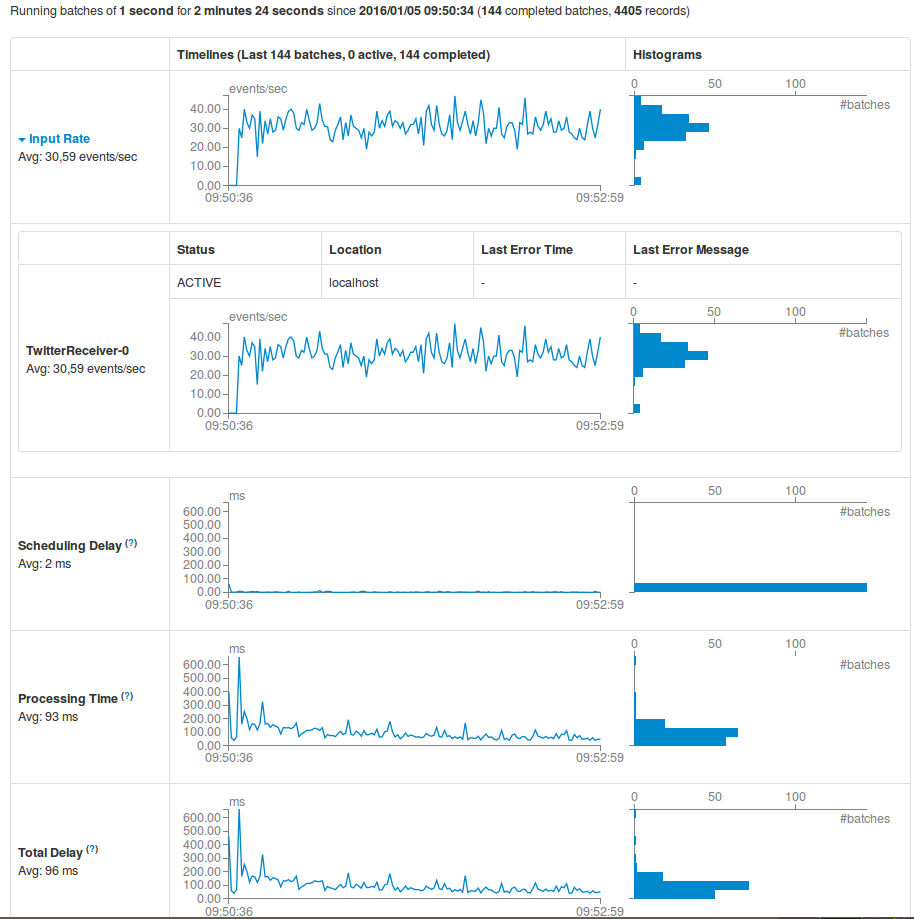
\includegraphics[width=1.0\textwidth]{images/streaming_spark_ui.png}
      \caption{Statistiques de Spark streaming}
      \label{fig:statistiques_spark_streaming_ui}
    \end{figure}

    Cependant, il serait intéressant de connaître la durée réelle de traitement d'un batch et non pas seulement la durée entre chaque batch qui est fixée manuellement. Spark possède une interface web regroupant de nombreuses métriques afin de suivre l'évolution de consommation de mémoire, le nombre de tâches effectuées, les erreurs… Ainsi la figure~\ref{fig:statistiques_spark_streaming_ui} présente ces résultats. La rubrique \emph{Processing Time} présente une moyenne de 104 ms pour traiter un batch dans son intégralité, ce qui est bien inférieur à la durée de 1s entre chaque batch et donc il n'y a pas de goulot d'étranglement. \\

    La deuxième métrique est nommée \emph{Statistics duration} est prend respectivement les valeurs 9, 21 et 19 millisecondes. Le temps de calcul des statistiques sur les tweets d'un batch est faible par rapport au temps de 104 ms nécessaire au traitement d'un batch. En effet, il y a peu de données à traiter et le temps restant est nécessaire au téléchargement des données depuis l'API de Twitter.

  \subsection{Resources utilization}
    \subsubsection{Vitesse de transmission}
      Une des métriques d'utilisation des ressources est la vitesse de transmission des messages entre l'API de Twitter et notre prototype. La figure~\ref{fig:statistiques_spark_streaming_ui} présente la catégorie \emph{Input Rate} qui correspond à la moyenne du nombre de Tweets par seconde. Cette valeur pour notre prototype est de 30,59 tweets par seconde.

    \subsubsection{Nombre d'erreurs}
      Une autre métrique était le nombre d'erreurs liés à la mémoire. La figure~\ref{fig:executor_spark_streaming_ui} présente des statistiques sur la mémoire des exécuteurs. Nous pouvons constater que la colonne \emph{Failed Tasks} a une valeur nulle et donc le prototype n'a pas eu d'erreur de mémoire.

      \begin{figure}
        \centering
        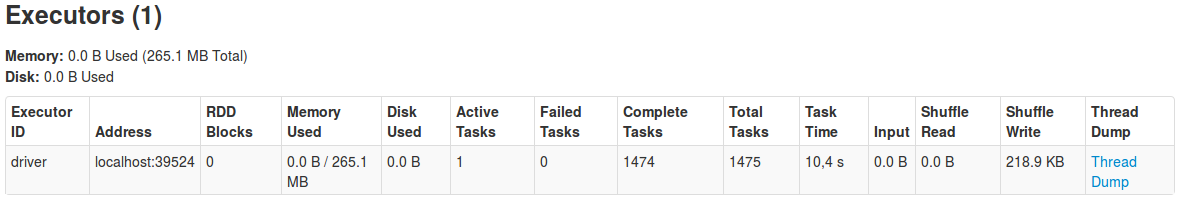
\includegraphics[width=1.0\textwidth]{images/executor_spark_ui.png}
        \caption{Statistiques liées à la mémoire}
        \label{fig:executor_spark_streaming_ui}
      \end{figure}

    \subsubsection{Pourcentage d'utilisation du CPU}
      Sur un ordinateur possédant un processeur Intel® Pentium(R) CPU P6100 @ 2.00GHz x 2, l'utilisation de notre prototype requiert 10\% du CPU.

  \subsection{Installability}
    \subsubsection{Installation du prototype}
      Afin d'utiliser le prototype, il est nécessaire d'installer 3 outils:
      \begin{itemize}
        \item Scala (\url{http://scala-lang.org/}), le langage utilisé pour l'implémentation du prototype
        \item Spark (\url{https://spark.apache.org/}), l'outil permettant le streaming avec l'API Twitter
        \item Sbt (\url{http://www.scala-sbt.org/}), un gestionnaire de dépendances
      \end{itemize}

    \subsubsection{Configuration du prototype}
      La seule étape de configuration du prototype est de récupérer les quatre tokens nécessaires à la connexion avec l'API de Twitter. La procédure est expliquée à cette adresse : \url{https://dev.twitter.com/oauth/overview/application-owner-access-tokens}.

    \subsubsection{Nombre de machine}
      L'utilisation de Spark streaming permet la gestion d'un nombre illimité de machines. Ainsi, plus le nombre de machines sera élevé et plus il sera possible de traiter un nombre de batch important, le tout avec un temps de traitement plus court. La procédure pour lancer le prototype sur un cluster de machine est disponible à cette adresse : \url{https://spark.apache.org/docs/latest/spark-standalone.html}.
